%%%%%%%%%%%%%%%%%%%%%%%%%%%%%%%%%%%%%%%%%%%%%%%%%%%%%%%%%%%%%%%%%%%%%%%%%%%%%%%
%  Mapping the Group--Individual Fairness Trade-off
%  IEEE conference format (IEEEtran, conference option)
%
%  COMPILE:  main.tex   (pdfLaTeX + BibTeX)
%  On Overleaf: Menu -> Compiler -> pdfLaTeX, then Recompile.
%%%%%%%%%%%%%%%%%%%%%%%%%%%%%%%%%%%%%%%%%%%%%%%%%%%%%%%%%%%%%%%%%%%%%%%%%%%%%%%
\documentclass[conference]{IEEEtran}
\IEEEoverridecommandlockouts

% ---- Bibliography / citation -------------------------------------------------
\usepackage{cite}

% ---- Math --------------------------------------------------------------------
\usepackage{amsmath,amssymb,amsfonts}

% ---- Algorithms --------------------------------------------------------------
\usepackage{algorithm}
\usepackage{algpseudocode}

% ---- Graphics and tables -----------------------------------------------------
\usepackage{graphicx}
\graphicspath{{figures/}}
\usepackage{booktabs}
\usepackage{multirow}
\usepackage{array}
\usepackage{xcolor}
\usepackage{textcomp}

% ---- Diagrams ----------------------------------------------------------------
\usepackage{tikz}
\usetikzlibrary{shapes.geometric,arrows.meta,positioning,calc}

% ---- URLs (loaded last among link-ish packages) ------------------------------
\usepackage{url}
\urlstyle{same}

% ---- Convenience macros ------------------------------------------------------
\newcommand{\dpdtwo}{\ensuremath{\mathrm{DPD}_{2}}}
\newcommand{\getwo}{\ensuremath{\mathrm{GE}(2)}}
\newcommand{\softdp}{\ensuremath{\mathcal{L}_{\mathrm{DP}}}}
\newcommand{\softge}{\ensuremath{\mathcal{L}_{\mathrm{GE}}}}
% compact "mean +- std" for wide tables: \ms{0.676}{0.012}
\newcommand{\ms}[2]{\ensuremath{#1_{\pm #2}}}
% significance marker
\newcommand{\sig}[1]{\textsuperscript{#1}}

% IEEEtran discourages \paragraph-style spacing changes; keep defaults.
\begin{document}

\title{Mapping the Group--Individual Fairness Trade-off:\\
An Empirical Study with a Differentiable Composite Loss}

\author{\IEEEauthorblockN{Tanushree Nepal}
\IEEEauthorblockA{\textit{Department of Computer Science and Cybersecurity} \\
\textit{University of Central Missouri}\\
Warrensburg, MO, USA \\
txn99360@ucmo.edu}
}

\maketitle

\begin{abstract}
Algorithmic fairness is not a single objective. \emph{Group} fairness asks
that demographic groups receive comparable treatment on average, while
\emph{individual} fairness asks that the burden of a model's errors be
distributed evenly across the people subject to it. Theoretical results
establish that such criteria are frequently incompatible, but the
\emph{magnitude} of the resulting trade-off on real data is far less
documented. We introduce a differentiable composite loss whose single
parameter $\beta$ interpolates continuously between a soft demographic-parity
term and a soft generalized-entropy term, and we use it as an instrument to
map the trade-off empirically. Sweeping a $7\times7$ grid over the
accuracy--fairness weight $\alpha$ and the group--individual weight $\beta$,
across three standard datasets (COMPAS, German Credit, Adult), two model
families (logistic regression and a multilayer perceptron), and ten random
seeds, we train and evaluate $2{,}940$ models. We observe a statistically
significant \emph{double dissociation}: optimizing the group term reduces the
demographic parity difference by up to $89\%$ but significantly worsens
individual-fairness inequality and, on Adult, degrades equalized odds by a
factor of $3.3$; optimizing the individual term significantly improves
individual fairness while leaving group disparity unchanged or slightly worse.
The composite loss attains group-fairness levels comparable to established
pre-, in-, and post-processing baselines. We further report a negative result
with a concrete diagnosis: on German Credit no effect survives significance
testing, and we show this is a failure of \emph{validation-based model
selection} at $n=1000$---validation and test demographic parity are
essentially uncorrelated ($r=0.08$, versus $0.94$ and $0.99$ on the other two
datasets)---rather than a failure of the method. Our results quantify a
trade-off that practitioners must resolve by policy, not by tuning.
\end{abstract}

\begin{IEEEkeywords}
algorithmic fairness, group fairness, individual fairness, demographic parity,
generalized entropy index, fairness--accuracy trade-off, differentiable
surrogate loss
\end{IEEEkeywords}

\section{Introduction}
\label{sec:intro}

Machine-learned models increasingly mediate consequential decisions about
people: whether a defendant is labelled high-risk, whether an applicant
receives credit, whether a r\'esum\'e is advanced. A decade of work has
established that such models can encode and amplify disparities present in
their training data~\cite{angwin2016machine,buolamwini2018gender,mehrabi2021survey}.
What is far less settled is what should be done about it---because
``fairness'' is not one property but a family of mutually inconsistent ones.

Two families dominate practice. \emph{Group fairness} requires that outcomes
be comparable across demographic groups; its canonical instance, demographic
parity, requires equal selection rates. \emph{Individual fairness} requires
that similar individuals be treated similarly~\cite{dwork2012fairness}, and in
its influential outcome-based operationalization requires that the
\emph{benefit} each person derives from the classifier be distributed evenly
across the population~\cite{speicher2018unified}. These are different
requirements, and satisfying one does not imply satisfying the other.

That they can conflict is known theoretically. Calibration and error-rate
balance cannot generally hold at once when base rates
differ~\cite{kleinberg2016inherent,chouldechova2017fair}; demographic parity
and equalized odds are likewise incompatible under the same
condition~\cite{barocas2019fairness}. What these results do \emph{not} supply
is a magnitude. A practitioner told that ``you cannot have both'' still needs
to know what one costs in units of the other, on data resembling their own,
with uncertainty quantified. Comparative empirical studies of fairness
interventions exist~\cite{friedler2019comparative}, but they typically compare
\emph{discrete methods}, each committed in advance to a single fairness
notion. What is missing is a study that varies the fairness objective
\emph{continuously} and measures both families of metrics along the way.

\subsection{Contributions}

We build such an instrument and use it to map the trade-off.

\begin{enumerate}
\item \textbf{A differentiable composite loss} (Section~\ref{sec:method}) whose
      parameter $\beta$ interpolates continuously between a soft
      demographic-parity term and a soft generalized-entropy term, with a
      second parameter $\alpha$ controlling the overall weight on fairness
      versus accuracy. Both fairness terms are computed on raw predicted
      probabilities so that gradients flow through them---the thresholding
      step that defines the evaluation metrics is not differentiable and
      cannot be optimized directly.
\item \textbf{An empirical trade-off map} (Section~\ref{sec:results}) built
      from a $7\times7$ $(\alpha,\beta)$ grid across three standard datasets,
      two model families, and ten seeds: $2{,}940$ trained models, all metrics
      reported as mean~$\pm$~standard deviation with paired significance tests.
\item \textbf{A statistically significant double dissociation.} Optimizing the
      group term reduces the demographic parity difference by $78\%$--$89\%$
      ($p_{\text{Holm}}=0.008$) while significantly \emph{worsening}
      individual-fairness inequality; optimizing the individual term
      significantly improves individual fairness while leaving group disparity
      unchanged or significantly worse. On Adult, driving demographic parity
      to near zero degrades equalized odds by a factor of $3.3$, an empirical
      instance of a known impossibility.
\item \textbf{A diagnosed negative result.} On German Credit no effect
      survives correction. We show this is not a failure of the method but of
      \emph{validation-based model selection at small $n$}: validation and
      test demographic parity are effectively uncorrelated
      ($r=0.08$ versus $0.94$ and $0.99$ elsewhere), so the selection rule
      cannot identify fair configurations. Under a pre-specified
      configuration the effect is present. We believe this sample-size floor
      on fairness model selection is of independent practical interest.
\item \textbf{A benchmark soundness correction.} We identify and remove a
      label-leaking feature from a COMPAS feature set in prior use, and report
      the honest accuracy that results.
\end{enumerate}

The composite loss is the \emph{instrument}; the trade-off map is the
\emph{contribution}. We do not claim a new state of the art in fairness
mitigation, and Section~\ref{sec:results} shows the loss matches rather than
beats established baselines on group-fairness metrics. Its value is that,
unlike those baselines, it exposes a continuous dial between two fairness
notions, which is precisely what mapping a trade-off requires.

\section{Related Work}
\label{sec:related}

\subsection{Group Fairness Criteria and Mitigation}

Group-fairness criteria constrain statistics of the prediction conditioned on
a sensitive attribute. \emph{Demographic parity} equalizes selection rates;
\emph{equalized odds} equalizes true- and false-positive rates across
groups~\cite{hardt2016equality}; \emph{equal opportunity} equalizes true
positive rates only. Surveys catalogue more than twenty such
definitions~\cite{verma2018fairness,mehrabi2021survey}, many of which cannot
hold simultaneously.

Mitigation methods are conventionally grouped into three families, all three
of which we use as baselines. \emph{Pre-processing} alters the training data:
reweighing assigns each sample a weight making label and sensitive attribute
independent in the weighted distribution~\cite{kamiran2012data}; related work
repairs feature distributions directly~\cite{feldman2015certifying} or learns
fair representations~\cite{zemel2013learning}. \emph{In-processing} alters the
objective, either by adding fairness constraints or penalties to the training
problem~\cite{zafar2017fairness}, by reduction to a sequence of cost-sensitive
problems~\cite{agarwal2018reductions}, or adversarially~\cite{zhang2018mitigating}.
\emph{Post-processing} adjusts a fixed model's outputs, typically via
group-dependent thresholds~\cite{hardt2016equality}. Our method is
in-processing; we compare against a representative of each family.

\subsection{Individual Fairness}

Dwork et al.~\cite{dwork2012fairness} formalize individual fairness as a
Lipschitz condition: individuals who are similar under a task-specific metric
must receive similar output distributions. The framework is principled but
requires a similarity metric that is rarely available in practice.

Speicher et al.~\cite{speicher2018unified} propose an outcome-based
alternative that requires no similarity metric. For each individual they
define a \emph{benefit} $b_i$ capturing how much that person received relative
to what they were owed, and then apply an inequality index from the economics
literature---the generalized entropy (GE) family~\cite{shorrocks1980class,cowell2011measuring}---to
the benefit vector. This unifies group and individual unfairness: the GE index
of the benefit vector decomposes additively into a between-group and a
within-group component. We adopt this operationalization, and we are explicit
throughout that it measures inequality of outcomes rather than the
Lipschitz condition of~\cite{dwork2012fairness}.

\subsection{Impossibility and Trade-off Results}

Kleinberg et al.~\cite{kleinberg2016inherent} and
Chouldechova~\cite{chouldechova2017fair} independently showed that
calibration, balance for the positive class, and balance for the negative
class cannot hold together unless base rates are equal or prediction is
perfect. Corbett-Davies et al.~\cite{corbett2017algorithmic} characterize the
cost of imposing parity constraints on a utility-maximizing decision rule.
Barocas et al.~\cite{barocas2019fairness} give the general statement that
independence (demographic parity) and separation (equalized odds) are
incompatible whenever the sensitive attribute and label are dependent---the
condition that holds in all three of our datasets.

These results establish existence, not magnitude, and they concern conflicts
\emph{within} group fairness. Our focus is the less-charted conflict
\emph{between} group and individual fairness, measured rather than derived.

\subsection{Empirical Comparisons and Benchmark Critique}

Friedler et al.~\cite{friedler2019comparative} benchmark fairness-enhancing
interventions across datasets and metrics, and emphasize that conclusions are
sensitive to preprocessing and train/test splits---motivating our per-seed
protocol. We extend this style of comparison along a new axis: rather than
comparing methods that each fix a fairness notion, we vary the notion
continuously within a single method.

A parallel literature critiques the benchmarks themselves. Bao et
al.~\cite{bao2021its} argue that COMPAS is routinely used in ways that
misrepresent the underlying criminal-justice process; Fabris et
al.~\cite{fabris2022algorithmic} survey the provenance of fairness datasets;
Ding et al.~\cite{ding2021retiring} document defects in the standard Adult
dataset and propose replacements. We contribute a concrete instance:
Section~\ref{sec:setup} identifies a label-leaking feature in a COMPAS feature
set and quantifies the inflated accuracy it produces.

\section{Method}
\label{sec:method}

\subsection{Problem Setting and Notation}

We consider binary classification. Let $x_i \in \mathbb{R}^d$ be the feature
vector of individual $i$, $y_i \in \{0,1\}$ the true label, and
$s_i \in \mathcal{S}$ the sensitive attribute, where $\mathcal{S}$ is a finite
set of demographic groups. A model $f_\theta$ produces a logit
$z_i = f_\theta(x_i)$, a probability $p_i = \sigma(z_i)$ with
$\sigma(\cdot)$ the logistic function, and a hard decision
$\hat{y}_i = \mathbf{1}[p_i \geq 0.5]$.

\subsection{Why a Surrogate Is Necessary}

The evaluation criteria of Section~\ref{sec:setup} are defined on the hard
decisions $\hat{y}_i$. The map $p_i \mapsto \mathbf{1}[p_i \geq 0.5]$ has zero
derivative almost everywhere and is undefined at the threshold, so any
objective written in terms of $\hat{y}$ has no usable gradient and cannot be
minimized by backpropagation. We therefore construct \emph{differentiable
surrogates} that operate on the probabilities $p_i$ directly, and verify
empirically (Section~\ref{sec:surrogate}) that each surrogate tracks the hard
metric it stands in for.

\subsection{Group Term: Soft Demographic Parity}

The demographic parity difference is the largest gap in selection rate between
any two groups. Replacing the selection rate with the mean predicted
probability gives a differentiable analogue:
\begin{equation}
\softdp(p, s) \;=\; \max_{g \in \mathcal{S}} \bar{p}_g \;-\; \min_{g \in \mathcal{S}} \bar{p}_g ,
\qquad
\bar{p}_g \;=\; \frac{1}{|\mathcal{I}_g|}\sum_{i \in \mathcal{I}_g} p_i ,
\label{eq:softdp}
\end{equation}
where $\mathcal{I}_g = \{ i : s_i = g \}$. Equation~\eqref{eq:softdp} is
differentiable in $\theta$ through $p$, and converges to the hard demographic
parity difference as the probabilities saturate towards $\{0,1\}$.

\subsection{Individual Term: Soft Generalized Entropy}

Following Speicher et al.~\cite{speicher2018unified} we define the
\emph{benefit} received by individual $i$ as
\begin{equation}
b_i \;=\; 1 + p_i - y_i .
\label{eq:benefit}
\end{equation}
A correctly served individual has $b_i \approx 1$; a false positive receives
more than deserved ($b_i \to 2$) and a false negative less ($b_i \to 0$).
Individual unfairness is then the \emph{inequality} of the benefit vector,
measured by the generalized entropy index of order $\gamma$:
\begin{equation}
\softge(p,y) \;=\; \frac{1}{n\,\gamma(\gamma-1)} \sum_{i=1}^{n}
\left[ \left( \frac{b_i}{\bar{b}} \right)^{\gamma} - 1 \right],
\label{eq:softge}
\end{equation}
where $\bar{b} = n^{-1}\sum_i b_i$ is the mean benefit.
We use $\gamma = 2$ throughout, for which \eqref{eq:softge} equals half the
squared coefficient of variation of $b$. The index is zero exactly when every
individual receives identical benefit, and grows as the burden of the model's
errors concentrates on fewer people. Because $b_i$ depends on $p_i$ smoothly,
\eqref{eq:softge} is differentiable.

\subsection{The Composite Loss}

The two fairness terms are combined with the accuracy term into a single
objective with two interpolation weights $\alpha, \beta \in [0,1]$:
\begin{equation}
\boxed{\;
\mathcal{L}(\theta)
= \alpha\,\mathcal{L}_{\mathrm{BCE}}
+ (1-\alpha)\Big[\beta\,\softdp + (1-\beta)\,\softge\Big] \;}
\label{eq:composite}
\end{equation}
where $\mathcal{L}_{\mathrm{BCE}}$ is binary cross-entropy computed from
logits for numerical stability. The two parameters have distinct roles:

\begin{itemize}
\item $\alpha$ trades \emph{accuracy against fairness}. At $\alpha=1$ the loss
      reduces to plain cross-entropy, giving the unconstrained baseline. As
      $\alpha \to 0$ accuracy is ignored entirely, which yields degenerate
      constant predictors (Section~\ref{sec:selection}).
\item $\beta$ trades \emph{group against individual fairness}, and is the
      variable of interest in this study. At $\beta=1$ the fairness budget is
      spent entirely on demographic parity; at $\beta=0$ entirely on benefit
      equality; intermediate values blend them.
\end{itemize}

Sweeping $\beta$ at fixed $\alpha$ therefore holds the total fairness pressure
constant while redistributing it between the two notions---which is exactly
the comparison needed to isolate a trade-off between them.

\subsection{Models}

We instantiate \eqref{eq:composite} with two model families, chosen to span a
linear and a nonlinear hypothesis class while remaining standard in the
fairness literature:
\begin{itemize}
\item \textbf{Logistic regression}: a single affine layer returning a logit.
\item \textbf{MLP (64--64)}: two hidden layers of 64 units with ReLU
      activations, returning a logit.
\end{itemize}
Both return logits rather than probabilities; the sigmoid is applied once,
inside the loss.

\subsection{Training and Selection Procedure}
\label{sec:selection}

Algorithm~\ref{alg:sweep} states the full procedure. Training uses
Adam~\cite{kingma2015adam} with learning rate $0.01$ and weight decay
$10^{-4}$, for at most $300$ epochs, with early stopping on the validation
value of the \emph{same} composite loss being optimized (patience $20$) and
restoration of the best weights from a deep copy. Because \eqref{eq:softdp}
requires all groups to be present in order to form a group gap, each epoch is
a single full-batch gradient step rather than a pass of mini-batches.

\begin{algorithm}[t]
\caption{$\alpha\times\beta$ sweep with validation-only selection}
\label{alg:sweep}
\begin{algorithmic}[1]
\Require dataset $D$, seed set $S$, grids $A$ (for $\alpha$), $B$ (for $\beta$)
\For{each seed $k \in S$}
  \State $(D_{\text{tr}},D_{\text{va}},D_{\text{te}}) \gets \textproc{Split}(D, 60/20/20, k)$
  \State fit scaler and encoder on $D_{\text{tr}}$; apply to all splits
  \For{each architecture $a$ and each $(\alpha,\beta) \in A \times B$}
     \State seed weights with $k$; initialise $f_\theta$
     \State train $f_\theta$ on $D_{\text{tr}}$ minimising \eqref{eq:composite}
     \State early-stop on $\mathcal{L}$ evaluated on $D_{\text{va}}$
     \State record test metrics, and validation accuracy,
            \dpdtwo{} and positive rate
  \EndFor
  \State \textbf{// selection uses validation quantities only}
  \State $F \gets \{(\alpha,\beta) : \alpha < 1,\;
         0.05 \le \widehat{r}_{\text{va}} \le 0.95 \}$
  \State $(\alpha^\ast,\beta^\ast) \gets
         \arg\min_{F} \sqrt{(1-\mathrm{acc}_{\text{va}})^2
         + \mathrm{DPD}_{2,\text{va}}^{2}}$
  \State report test metrics at $(\alpha^\ast,\beta^\ast)$
\EndFor
\State aggregate over $S$; paired Wilcoxon test with Holm correction
\end{algorithmic}
\end{algorithm}

Two details in Algorithm~\ref{alg:sweep} matter for the validity of the
results. First, \emph{test metrics are never used for selection}: the
$(\alpha,\beta)$ pair is chosen by distance to the utopia point
$(\text{accuracy}=1, \dpdtwo=0)$ computed on validation data alone. Second,
the constraint $0.05 \le \widehat{r}_{\text{va}} \le 0.95$ on the validation
positive rate $\widehat{r}_{\text{va}}$ excludes near-constant predictors: a
model that assigns every individual to one class attains
$\dpdtwo = 0$ trivially while being useless. This guard is not cosmetic---at
$\alpha=0$ we observe validation positive rates above $0.99$.

\subsection{Pipeline Overview}

Fig.~\ref{fig:pipeline} summarizes the complete experimental pipeline from raw
data to reported results.

\begin{figure}[t]
\centering
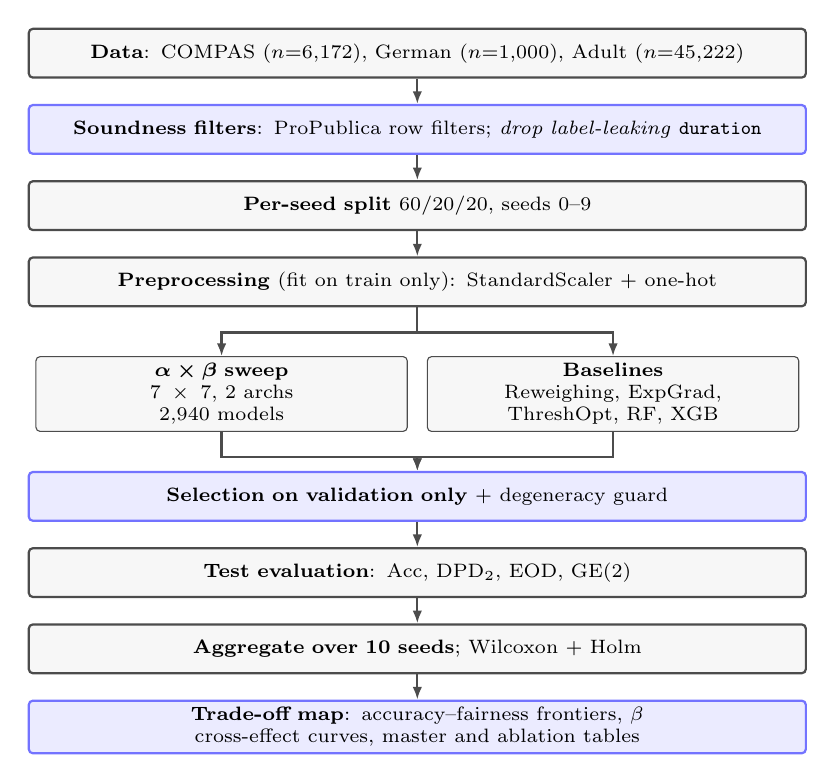
\begin{tikzpicture}[
  node distance=3.2mm,
  every node/.style={font=\scriptsize},
  box/.style={rectangle, rounded corners=1.5pt, draw=black!70, thick,
              text width=0.80\columnwidth, align=center, inner sep=2.4pt,
              minimum height=6.2mm, fill=black!3},
  hi/.style={box, fill=blue!8, draw=blue!55},
  sm/.style={rectangle, rounded corners=1.5pt, draw=black!70,
             text width=0.375\columnwidth, align=center, inner sep=2.4pt,
             minimum height=8.5mm, fill=black!3},
  ar/.style={-{Latex[length=1.6mm]}, thick, draw=black!70}
]
\node[box] (data) {\textbf{Data}: COMPAS ($n{=}6{,}172$), German ($n{=}1{,}000$),
                   Adult ($n{=}45{,}222$)};
\node[hi, below=of data] (filt) {\textbf{Soundness filters}: ProPublica row
                   filters; \emph{drop label-leaking} \texttt{duration}};
\node[box, below=of filt] (split) {\textbf{Per-seed split} $60/20/20$,
                   seeds $0$--$9$};
\node[box, below=of split] (prep) {\textbf{Preprocessing} (fit on train only):
                   StandardScaler $+$ one-hot};
\node[sm] (sweep) at ([xshift=-0.205\columnwidth, yshift=-11mm]prep.south)
      {$\boldsymbol{\alpha\times\beta}$ \textbf{sweep}\\
       $7\times7$, 2 archs\\ $2{,}940$ models};
\node[sm] (base)  at ([xshift= 0.205\columnwidth, yshift=-11mm]prep.south)
      {\textbf{Baselines}\\ Reweighing, ExpGrad,\\ ThreshOpt, RF, XGB};
\node[hi] (sel) at ([yshift=-24mm]prep.south)
                  {\textbf{Selection on validation only}
                   $+$ degeneracy guard};
\node[box, below=of sel] (eval) {\textbf{Test evaluation}: Acc, \dpdtwo{},
                   EOD, \getwo{}};
\node[box, below=of eval] (agg) {\textbf{Aggregate over 10 seeds};
                   Wilcoxon $+$ Holm};
\node[hi, below=of agg] (res) {\textbf{Trade-off map}:
                   accuracy--fairness frontiers, $\beta$ cross-effect curves,
                   master and ablation tables};

\draw[ar] (data) -- (filt);
\draw[ar] (filt) -- (split);
\draw[ar] (split) -- (prep);
\draw[ar] (prep.south) -- ++(0,-3.2mm) -| (sweep.north);
\draw[ar] (prep.south) -- ++(0,-3.2mm) -| (base.north);
\draw[ar] (sweep.south) |- ([yshift=-3.2mm]sweep.south) -| (sel.north);
\draw[ar] (base.south)  |- ([yshift=-3.2mm]base.south)  -| (sel.north);
\draw[ar] (sel) -- (eval);
\draw[ar] (eval) -- (agg);
\draw[ar] (agg) -- (res);
\end{tikzpicture}
\caption{Experimental pipeline. Shaded boxes mark the three steps that most
affect the validity of the conclusions: removal of the label-leaking COMPAS
feature, selection performed strictly on validation data with a
degenerate-predictor guard, and reporting of the resulting trade-off map.}
\label{fig:pipeline}
\end{figure}

\section{Experimental Setup}
\label{sec:setup}

\subsection{Datasets}

We use three datasets that together span three application domains, two
sensitive attributes, and one and a half orders of magnitude in sample size.
Table~\ref{tab:datasets} reports their characteristics after filtering.

\begin{table}[t]
\caption{Dataset characteristics after filtering. Base rates are the fraction
of positive labels. The positive class is the \emph{adverse} outcome for
COMPAS and German Credit and the \emph{favourable} outcome for Adult.}
\label{tab:datasets}
\centering
\footnotesize
\setlength{\tabcolsep}{3.2pt}
\begin{tabular}{@{}lccc@{}}
\toprule
 & \textbf{COMPAS} & \textbf{German} & \textbf{Adult} \\
\midrule
Samples $n$              & $6{,}172$ & $1{,}000$ & $45{,}222$ \\
Encoded features $d$     & $12$      & $21$      & $79$ \\
Target ($y=1$)           & re-offend & bad credit & income $>\!50$K \\
Sensitive attribute      & race      & sex        & sex \\
Groups $|\mathcal{S}|$   & $6$       & $2$        & $2$ \\
Overall base rate        & $0.455$   & $0.300$    & $0.248$ \\
\midrule
\multicolumn{4}{@{}l}{\textit{Two largest groups (size; base rate)}}\\
Group 1 & Afr.-Am. & male & Male \\
        & ($3{,}175$; $0.523$) & ($690$; $0.277$) & ($30{,}527$; $0.312$) \\
Group 2 & Caucasian & female & Female \\
        & ($2{,}103$; $0.391$) & ($310$; $0.352$) & ($14{,}695$; $0.114$) \\
\bottomrule
\end{tabular}
\end{table}

Base rates differ across groups in all three datasets, most sharply in Adult
($0.312$ versus $0.114$, a factor of $2.7$). This is the precise condition
under which demographic parity and equalized odds are provably
incompatible~\cite{barocas2019fairness}, and it drives the result of
Section~\ref{sec:adult}.

\subsubsection{COMPAS and a label-leakage correction}
We apply ProPublica's standard row filters~\cite{angwin2016machine}
(screening date within $\pm 30$ days of arrest, valid recidivism flag,
charge degree not ordinary, valid score text) and use their standard feature
set: age, sex, juvenile felony/misdemeanour/other counts, prior counts, charge
degree, and race.

A feature set previously used in our own pipeline additionally contained
$\texttt{duration} = \texttt{end} - \texttt{start}$, the length of the
observation window. This feature correlates $-0.78$ with the target for a
\emph{mechanical} reason: re-offending truncates the observation window, so a
short duration nearly implies the positive label. It is label leakage rather
than signal, and we remove it. Doing so lowers COMPAS accuracy to
approximately $0.68$, consistent with the literature; we regard the lower
number as the correct one and report it throughout.

\subsubsection{German Credit}
We take the Statlog encoding~\cite{hofmann1994statlog} and define $y=1$ as
\emph{bad} credit risk, so that---as in COMPAS---the positive class is the
adverse outcome.

\subsubsection{Adult}
We use the $48{,}842$-row version~\cite{uci2017adult}, drop rows with missing
values, exclude
\texttt{fnlwgt} (a census sampling weight, not a person-level attribute), and
prefer the ordinal \texttt{education-num} over the redundant categorical
\texttt{education}.

The sensitive attribute is retained as a model input in all cases. This is a
deliberate ``fairness through awareness'' choice~\cite{dwork2012fairness}:
removing it does not remove the information, since correlated proxies remain,
and withholding it would prevent the group term \eqref{eq:softdp} from being
expressed.

\subsection{Preprocessing and Protocol}

Each seed $k \in \{0,\dots,9\}$ draws an independent $60/20/20$
train/validation/test split and initialises model weights. Numeric features
are standardised and categorical features one-hot encoded with the first level
dropped; unseen categories at transform time are encoded as all-zeros. All
transformers are fit on the training split only. Splits are not stratified.

Ten seeds give ten paired observations per comparison. All results are
reported as mean $\pm$ standard deviation over seeds.

\subsection{Evaluation Metrics}

We evaluate on hard test predictions at a fixed threshold of $0.5$.

\subsubsection{Accuracy} Fraction of correct predictions. Higher is better.
There is no universal target; the relevant reference points are the
majority-class rate and dataset-typical published performance.

\subsubsection{Demographic parity difference (DPD)}
The largest gap in selection rate between groups,
$\max_g P(\hat{y}=1 \mid S=g) - \min_g P(\hat{y}=1 \mid S=g)$. Lower is
better; the range is $[0,1]$. We emphasize \dpdtwo{}, the same quantity
computed on the two \emph{largest} groups only. On COMPAS the all-groups
statistic is pinned by groups of $31$ and $11$ individuals (roughly $6$ and
$2$ in a test split), making it extremely unstable: across seeds we measure
$0.608 \pm 0.211$ for the all-groups version against $0.304 \pm 0.049$ for
\dpdtwo{}, a fourfold reduction in variance. For German and Adult, which have
two groups, the two statistics coincide by construction.

\subsubsection{Equalized odds difference (EOD)}
The larger of the between-group true-positive-rate gap and the
false-positive-rate gap~\cite{hardt2016equality}. Lower is better. Unlike DPD
it conditions on the true label.

\subsubsection{Generalized entropy index, \getwo{}}
Equation~\eqref{eq:softge} evaluated on hard predictions, i.e. the inequality
of the benefit vector \eqref{eq:benefit} with $b_i \in \{0,1,2\}$. Lower is
better, with $0$ attained only by a perfect classifier.

We note explicitly that no threshold in the literature designates a ``fair''
value of DPD, EOD, or \getwo{}. The four-fifths rule~\cite{eeoc1978uniform} is
sometimes invoked, but it is a \emph{ratio} test on selection rates and does
not translate into a difference threshold. Values such as $\mathrm{DPD}<0.05$
are conventions of practice, not standards. \getwo{} has no absolute
interpretation at all and is meaningful only in comparison between models on
the same data. We therefore report all comparisons as differences against a
matched baseline with significance tests, rather than against absolute cutoffs.

\subsection{Baselines}

We compare against one representative from each mitigation family plus two
unconstrained accuracy references, all fit on the same per-seed split:

\begin{itemize}
\item \textbf{Reweighing}~\cite{kamiran2012data} (pre-processing): logistic
      regression trained with sample weights
      $w(s,y) = P(s)P(y)/P(s,y)$.
\item \textbf{ExponentiatedGradient}~\cite{agarwal2018reductions}
      (in-processing), with demographic-parity and with equalized-odds
      constraints.
\item \textbf{ThresholdOptimizer}~\cite{hardt2016equality} (post-processing),
      demographic-parity constraint, group-specific thresholds.
\item \textbf{Random Forest} ($300$ trees) and
      \textbf{XGBoost}~\cite{chen2016xgboost} ($300$ estimators, depth $6$,
      learning rate $0.1$): no fairness intervention; these establish the
      accuracy ceiling.
\end{itemize}

\subsection{Statistical Testing}

For each (fair model, baseline) pair we apply a paired Wilcoxon signed-rank
test~\cite{wilcoxon1945individual} across the ten seeds---paired because both
models see identical splits, non-parametric because ten observations do not
justify a normality assumption~\cite{demsar2006statistical}. We correct across
the four-metric family $\{$accuracy, \dpdtwo{}, EOD, \getwo{}$\}$ using the
Holm step-down procedure~\cite{holm1979simple}. With $n=10$ the smallest
attainable two-sided $p$-value is $2^{-9} \approx 0.002$, which we report as
$p = 0.002$ rather than as an open bound.

\subsection{Implementation}

Models and the composite loss are implemented in
PyTorch~\cite{paszke2019pytorch}; preprocessing, logistic regression and
random forests use scikit-learn~\cite{pedregosa2011scikit}; group-fairness
metrics and the ExponentiatedGradient and ThresholdOptimizer baselines use
Fairlearn~\cite{bird2020fairlearn}; the generalized entropy index uses
AI Fairness 360~\cite{bellamy2019ai}. The full grid is
$7 \times 7$ values of $(\alpha,\beta)$ with
$\alpha,\beta \in \{0, 0.005, 0.05, 0.25, 0.5, 0.75, 1\}$, over $2$
architectures, $3$ datasets and $10$ seeds: $2{,}940$ trained models. All runs
are CPU-only.

\section{Results}
\label{sec:results}

\subsection{Surrogate Validation}
\label{sec:surrogate}

Because training minimises the soft surrogates \eqref{eq:softdp} and
\eqref{eq:softge} while evaluation uses hard-threshold metrics, we first check
that the two agree. Fig.~\ref{fig:surrogate} plots each surrogate against the
metric it stands in for, over all $2{,}940$ models.

\begin{figure}[t]
\centering
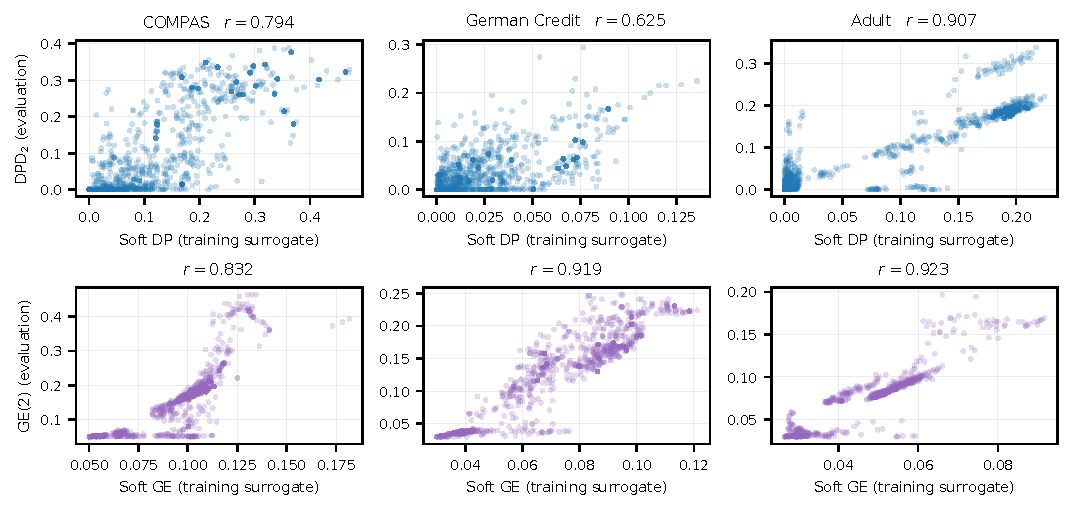
\includegraphics[width=\columnwidth]{surrogate_validation.pdf}
\caption{Training surrogate versus hard evaluation metric, all sweep points
and all seeds. Top: \softdp{} against \dpdtwo{}. Bottom: \softge{} against
\getwo{}. Correlations are strong on COMPAS and Adult; the weaker
$r=0.625$ for \softdp{} on German reflects that dataset's $200$-row test
split rather than a defect of the surrogate.}
\label{fig:surrogate}
\end{figure}

Pearson correlations are $r = 0.794$ (COMPAS), $0.625$ (German) and $0.907$
(Adult) for $\softdp \leftrightarrow \dpdtwo$, and $0.832$, $0.919$, $0.923$
for $\softge \leftrightarrow \getwo$. The surrogates track their targets, with
German's group surrogate the weakest link---an early indication of the
small-sample behaviour analysed in Section~\ref{sec:german}.

\subsection{RQ1: A Double Dissociation Between the Two Objectives}
\label{sec:rq1}

The cleanest test of a trade-off holds the total fairness weight fixed and
moves only $\beta$. Table~\ref{tab:ablation} does this at the selected
$\alpha^\ast$, comparing the two extremes---individual-only ($\beta=0$) and
group-only ($\beta=1$)---against the unconstrained $\alpha=1$ baseline.
Fig.~\ref{fig:dissociation} shows the same contrast as percentage change.

\begin{figure}[t]
\centering
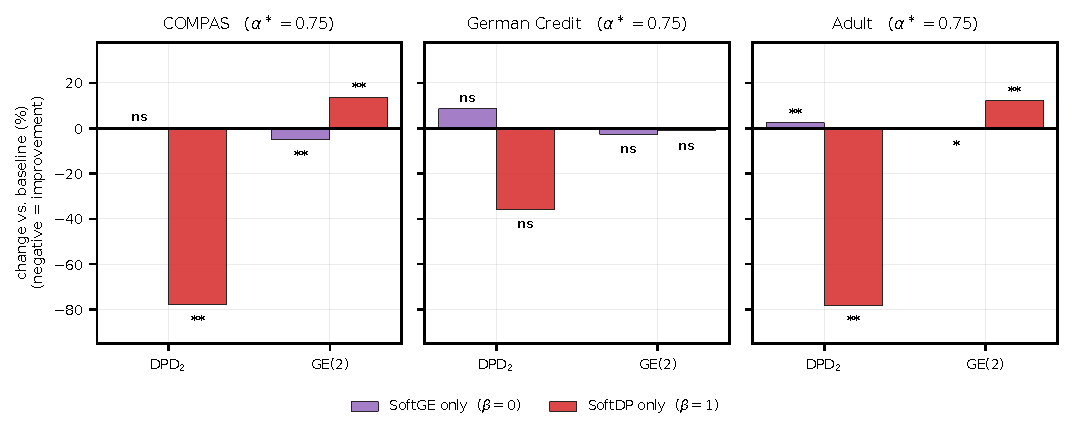
\includegraphics[width=\columnwidth]{double_dissociation.pdf}
\caption{Percentage change from the unconstrained baseline when the fairness
budget is spent entirely on the individual term ($\beta=0$, purple) or
entirely on the group term ($\beta=1$, red), logistic regression. The two
objectives improve the metric they target and leave or push the other in the
wrong direction. Markers give Holm-corrected paired Wilcoxon significance
($^{**}p<0.01$, $^{*}p<0.05$, ns $=$ not significant).}
\label{fig:dissociation}
\end{figure}

The pattern is a double dissociation and it is consistent on the two datasets
with a disparity to act on:

\begin{itemize}
\item \textbf{Group objective ($\beta=1$)} reduces \dpdtwo{} by $78\%$ on
      COMPAS ($0.304 \to 0.067$) and $78\%$ on Adult ($0.184 \to 0.040$),
      both $p_{\text{Holm}}=0.008$. It simultaneously \emph{worsens} \getwo{}
      ($0.191 \to 0.217$ on COMPAS, $0.084 \to 0.094$ on Adult), both
      $p_{\text{Holm}}=0.008$---i.e. worse individual fairness than doing
      nothing at all.
\item \textbf{Individual objective ($\beta=0$)} improves \getwo{}
      ($0.191 \to 0.181$ on COMPAS, $0.084 \to 0.083$ on Adult, both
      $p_{\text{Holm}} \le 0.012$) but does not improve \dpdtwo{}: it is
      statistically unchanged on COMPAS ($0.304 \to 0.305$, $p=0.85$) and
      significantly \emph{worse} on Adult ($0.184 \to 0.189$,
      $p_{\text{Holm}}=0.008$).
\end{itemize}

The effects are asymmetric in size: the group term moves its target by nearly
$80\%$, the individual term by around $5\%$. We interpret this in
Section~\ref{sec:discussion}.

\subsection{RQ2: Consistency Across Datasets and Architectures}

Fig.~\ref{fig:beta} traces both metrics continuously across $\beta$ at fixed
$\alpha=0.75$. On COMPAS and Adult, and for both architectures, the two curves
cross: as $\beta$ increases the group metric falls monotonically while the
individual metric rises monotonically. The MLP reproduces the logistic
regression pattern closely, indicating the tension is not an artefact of a
linear hypothesis class.

\begin{figure}[t]
\centering
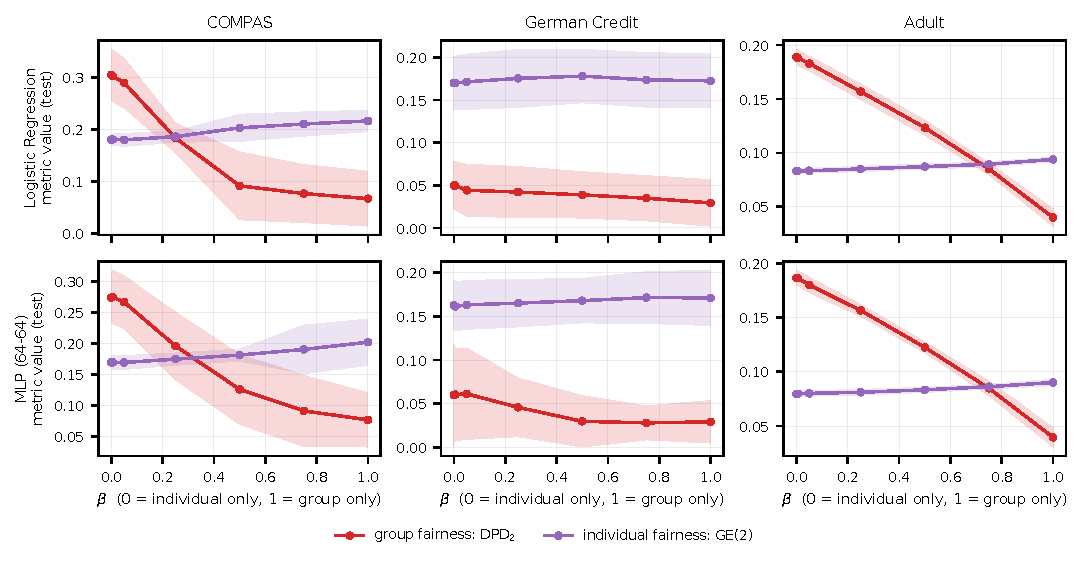
\includegraphics[width=\columnwidth]{beta_cross_effect.pdf}
\caption{Group fairness (\dpdtwo{}, red) and individual fairness (\getwo{},
purple) as $\beta$ moves from individual-only ($0$) to group-only ($1$), at
$\alpha=0.75$. Bands are $\pm 1$ standard deviation over ten seeds. The
crossing curves on COMPAS and Adult are the trade-off; German Credit is flat
because its baseline disparity is already small.}
\label{fig:beta}
\end{figure}

Fig.~\ref{fig:tradeoff} views the same data as a frontier in
(\dpdtwo{}, \getwo{}) space, with $\beta$ encoded by colour: configurations
sort along a diagonal from low-\getwo{}/high-\dpdtwo{} to
high-\getwo{}/low-\dpdtwo{}. Appendix heatmaps
(Figs.~\ref{fig:heatdpd}--\ref{fig:heatge}) show the full $\alpha \times \beta$
surface for both metrics.

\begin{figure}[t]
\centering
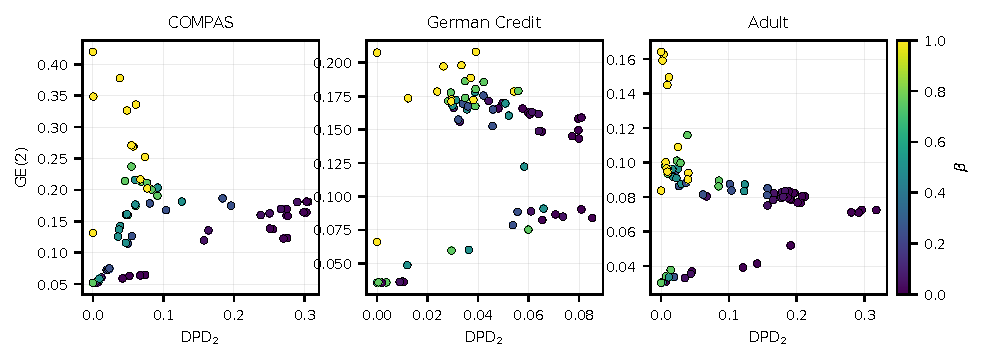
\includegraphics[width=\columnwidth]{dpd_vs_ge_tradeoff.pdf}
\caption{Group versus individual fairness across all $\alpha<1$ sweep points
(seed means), coloured by $\beta$. Points order along the diagonal by $\beta$,
tracing the attainable trade-off surface.}
\label{fig:tradeoff}
\end{figure}

\subsection{The Adult Parity--Odds Inversion}
\label{sec:adult}

Adult exhibits the trade-off in its sharpest form, involving two \emph{group}
criteria. Driving demographic parity down drives equalized odds up: for the
MLP at $\beta=1$, \dpdtwo{} falls from $0.182$ to $0.009$---essentially
perfect demographic parity---while EOD rises from $0.097$ to $0.321$, a factor
of $3.3$ (both $p_{\text{Holm}}=0.008$). For logistic regression the same
contrast gives $0.184 \to 0.040$ on \dpdtwo{} against $0.107 \to 0.246$ on EOD.

This is the empirical face of a known impossibility. Adult's group base rates
differ by a factor of $2.7$ (Table~\ref{tab:datasets}), and under unequal base
rates independence and separation cannot hold
together~\cite{barocas2019fairness}. The contribution here is the exchange
rate: on this dataset roughly one point of demographic parity is bought with
$1.1$ points of equalized odds. A model can therefore be made near-perfectly
``fair'' under one standard definition while becoming markedly less fair under
another, and the reported number depends entirely on which definition the
deploying institution has adopted.

\subsection{RQ3: Comparison Against Established Baselines}

Table~\ref{tab:master} reports every method on every dataset, and
Fig.~\ref{fig:pareto} places the full sweep and the baselines in
accuracy--\dpdtwo{} space.

\begin{figure}[t]
\centering
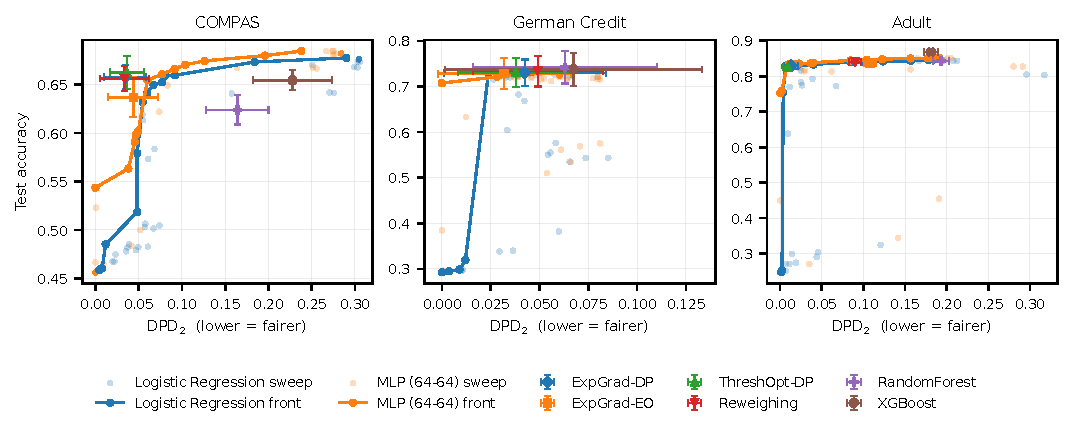
\includegraphics[width=\columnwidth]{pareto_frontiers.pdf}
\caption{Accuracy versus \dpdtwo{} (seed means). Faint points are individual
sweep configurations; solid lines are the Pareto fronts per architecture;
markers with error bars are the baselines ($\pm 1$ std over seeds). The
composite-loss front reaches the same region as the dedicated
group-fairness baselines.}
\label{fig:pareto}
\end{figure}

The honest reading is that the composite loss is \emph{competitive but not
superior} on group fairness. On COMPAS at comparable accuracy, Reweighing
reaches $\dpdtwo=0.034$ and ExponentiatedGradient $0.035$, against $0.061$ for
our selected model; on Adult, ThresholdOptimizer reaches $0.009$ and
ExponentiatedGradient $0.013$, against $0.021$. Our MLP at
$(0.836, 0.026)$ is nonetheless on the joint frontier, being more accurate
than every baseline that achieves lower disparity.

Two further observations are worth recording. First, the accuracy ceiling on
Adult belongs to XGBoost at $0.868$, which also carries one of the largest
disparities ($\dpdtwo = 0.181$)---the most accurate model is among the least
fair. Second, ExponentiatedGradient with an equalized-odds constraint behaves
on Adult exactly as the inversion of Section~\ref{sec:adult} predicts, in
mirror image: it attains the best EOD of any method ($0.035$) while leaving
\dpdtwo{} at $0.108$, an order of magnitude above the parity-constrained
methods.

\subsection{RQ2 Continued: The German Credit Null Result and Its Cause}
\label{sec:german}

On German Credit, no comparison between a selected fair model and its baseline
survives Holm correction on any metric for either architecture (all
$p_{\text{Holm}} \geq 0.42$; see Fig.~\ref{fig:fairvsbase}). We report this as
a negative result and diagnose it, because the cause is not that the method
fails.

\begin{figure}[t]
\centering
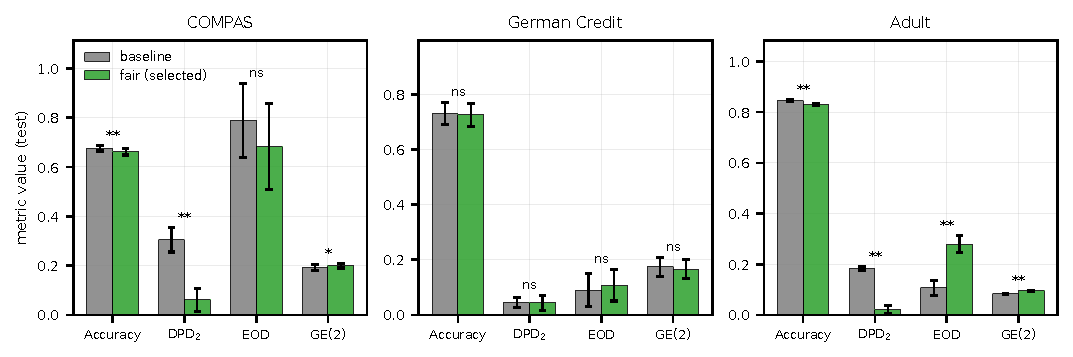
\includegraphics[width=\columnwidth]{fair_vs_baseline.pdf}
\caption{Selected fair logistic regression against its unconstrained baseline
(mean $\pm$ std over ten seeds), with Holm-corrected paired Wilcoxon markers.
COMPAS and Adult show significant reductions in \dpdtwo{}; German shows no
significant change on any metric.}
\label{fig:fairvsbase}
\end{figure}

Two mechanisms combine, and Table~\ref{tab:selection} quantifies both.

\subsubsection{Validation demographic parity is uninformative at $n=1000$}
Selection ranks configurations by validation \dpdtwo{}. On German that
quantity is essentially uncorrelated with the test value it is meant to
predict ($r = 0.08$ for logistic regression, $0.11$ for the MLP), against
$r \geq 0.89$ on COMPAS and $r \geq 0.99$ on Adult
(Fig.~\ref{fig:selection}). With a $200$-row validation split containing
roughly $62$ women, the standard error of a group selection rate is about
$\pm 0.04$---the size of the entire signal. The between-configuration spread
is smaller than the within-configuration seed noise
(signal-to-noise $0.45$ versus $1.68$ and $12.9$). Selection is therefore
ranking noise.

\begin{figure}[t]
\centering
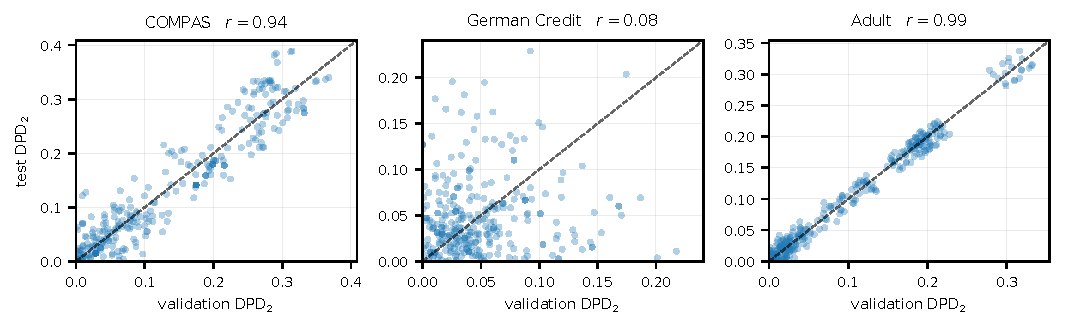
\includegraphics[width=\columnwidth]{selection_diagnostic.pdf}
\caption{Validation versus test \dpdtwo{} across all non-degenerate sweep
configurations (logistic regression). Dashed line is $y=x$. Validation
demographic parity predicts its test counterpart on COMPAS and Adult but
carries almost no information on German Credit.}
\label{fig:selection}
\end{figure}

\subsubsection{The selection criterion is scale-sensitive}
The utopia distance
$\sqrt{(1-\mathrm{acc})^2 + \mathrm{DPD}_2^2}$ weights an accuracy point and a
disparity point equally. That is reasonable when the two terms are comparable,
as on COMPAS ($1.1\times$) and Adult ($0.7\times$), but on German the accuracy
term exceeds the disparity term by a factor of $34.9$. The criterion
degenerates to ``maximise accuracy'' and is nearly blind to fairness even
before noise is considered. Consistent with this, the selected $\beta$
averages only $0.19$ on German---with three of ten seeds selecting
$\beta = 0$, i.e. no group-fairness weight at all---against $0.63$ on COMPAS
and $0.58$ on Adult, and the selected configuration differs across $8$ of $10$
seeds.

\subsubsection{The effect exists under a pre-specified configuration}
Bypassing selection entirely and fixing the group-fairness extreme
$\beta=1$, German logistic regression attains
$\dpdtwo = 0.024$ against a baseline $0.046$---a $48\%$ reduction---at
\emph{no} accuracy cost ($0.729$ versus $0.730$), improving in $8$ of $10$
seeds ($p = 0.020$, uncorrected). The pre-specified ablation contrast in
Table~\ref{tab:ablation} shows the same direction ($0.046 \to 0.029$) though
it does not survive correction. We conclude that the method reduces disparity
on German, and that validation-based selection at this sample size cannot
find the configurations that do so.

% ---------------------------------------------------------------- Table: master
\begin{table*}[t]
\caption{Master comparison. Mean $\pm$ standard deviation over ten seeds,
written $x_{\pm\sigma}$. Arrows give the preferred direction. \dpdtwo{} is the
demographic parity difference on the two largest groups; for German and Adult
it coincides with the all-groups value. Best value per column among all
methods is in \textbf{bold}. Baseline families: Reweighing is
pre-processing, ExpGrad in-processing, ThreshOpt post-processing. Fair models select $(\alpha,\beta)$ on validation
data only.}
\label{tab:master}
\centering
\scriptsize
\setlength{\tabcolsep}{2.25pt}
\begin{tabular}{@{}l cccc cccc cccc@{}}
\toprule
& \multicolumn{4}{c}{\textbf{COMPAS} (race)}
& \multicolumn{4}{c}{\textbf{German Credit} (sex)}
& \multicolumn{4}{c}{\textbf{Adult} (sex)} \\
\cmidrule(lr){2-5}\cmidrule(lr){6-9}\cmidrule(lr){10-13}
\textbf{Method}
& Acc$\uparrow$ & \dpdtwo{}$\downarrow$ & EOD$\downarrow$ & \getwo{}$\downarrow$
& Acc$\uparrow$ & \dpdtwo{}$\downarrow$ & EOD$\downarrow$ & \getwo{}$\downarrow$
& Acc$\uparrow$ & \dpdtwo{}$\downarrow$ & EOD$\downarrow$ & \getwo{}$\downarrow$ \\
\midrule
\multicolumn{13}{@{}l}{\textit{Unconstrained baselines}}\\
Logistic regression
& \ms{.676}{.012} & \ms{.304}{.049} & \ms{.789}{.151} & \ms{.191}{.012}
& \ms{.730}{.040} & \ms{.046}{.018} & \textbf{\ms{.090}{.059}} & \ms{.175}{.035}
& \ms{.845}{.004} & \ms{.184}{.007} & \ms{.107}{.030} & \ms{.084}{.002} \\
MLP (64--64)
& \textbf{\ms{.682}{.014}} & \ms{.284}{.044} & \ms{.829}{.151} & \textbf{\ms{.177}{.011}}
& \ms{.724}{.034} & \ms{.060}{.052} & \ms{.106}{.064} & \ms{.164}{.027}
& \ms{.851}{.004} & \ms{.182}{.008} & \ms{.097}{.024} & \ms{.080}{.003} \\
Random Forest
& \ms{.624}{.015} & \ms{.164}{.036} & \ms{.808}{.205} & \ms{.195}{.011}
& \textbf{\ms{.742}{.036}} & \ms{.063}{.047} & \ms{.133}{.086} & \ms{.156}{.027}
& \ms{.843}{.002} & \ms{.193}{.009} & \ms{.104}{.021} & \ms{.083}{.001} \\
XGBoost
& \ms{.655}{.010} & \ms{.228}{.045} & \ms{.791}{.181} & \ms{.196}{.011}
& \ms{.738}{.036} & \ms{.067}{.066} & \ms{.152}{.102} & \textbf{\ms{.148}{.024}}
& \textbf{\ms{.868}{.003}} & \ms{.181}{.008} & \ms{.087}{.023} & \textbf{\ms{.070}{.002}} \\
\midrule
\multicolumn{13}{@{}l}{\textit{This work: composite loss}}\\
Fair LogReg (ours)
& \ms{.661}{.013} & \ms{.061}{.047} & \ms{.683}{.173} & \ms{.200}{.010}
& \ms{.725}{.040} & \ms{.044}{.027} & \ms{.107}{.057} & \ms{.166}{.035}
& \ms{.830}{.003} & \ms{.021}{.016} & \ms{.279}{.034} & \ms{.095}{.002} \\
Fair MLP (ours)
& \ms{.669}{.018} & \ms{.082}{.047} & \ms{.766}{.181} & \ms{.181}{.014}
& \ms{.716}{.035} & \ms{.069}{.052} & \ms{.127}{.082} & \ms{.162}{.036}
& \ms{.836}{.004} & \ms{.026}{.015} & \ms{.281}{.031} & \ms{.091}{.003} \\
\midrule
\multicolumn{13}{@{}l}{\textit{Established mitigation baselines}}\\
Reweighing
& \ms{.656}{.013} & \textbf{\ms{.034}{.029}} & \textbf{\ms{.644}{.137}} & \ms{.205}{.011}
& \ms{.734}{.034} & \ms{.049}{.033} & \ms{.118}{.078} & \ms{.162}{.025}
& \ms{.840}{.003} & \ms{.090}{.007} & \ms{.149}{.029} & \ms{.088}{.002} \\
ExpGrad (DP)
& \ms{.658}{.012} & \ms{.035}{.024} & \ms{.766}{.216} & \ms{.200}{.010}
& \ms{.730}{.030} & \ms{.042}{.042} & \ms{.104}{.086} & \ms{.163}{.022}
& \ms{.830}{.003} & \ms{.013}{.008} & \ms{.300}{.014} & \ms{.096}{.002} \\
ExpGrad (EO)
& \ms{.637}{.021} & \ms{.044}{.029} & \ms{.737}{.206} & \ms{.206}{.015}
& \ms{.728}{.034} & \textbf{\ms{.032}{.034}} & \ms{.106}{.054} & \ms{.164}{.025}
& \ms{.836}{.004} & \ms{.108}{.007} & \textbf{\ms{.035}{.015}} & \ms{.090}{.003} \\
ThreshOpt (DP)
& \ms{.663}{.017} & \ms{.037}{.020} & \ms{.781}{.208} & \ms{.181}{.010}
& \ms{.731}{.032} & \ms{.038}{.029} & \ms{.129}{.060} & \ms{.162}{.025}
& \ms{.827}{.003} & \textbf{\ms{.009}{.006}} & \ms{.333}{.021} & \ms{.097}{.003} \\
\bottomrule
\end{tabular}
\end{table*}

% ------------------------------------------------------------- Table: ablation
\begin{table*}[t]
\caption{Ablation over $\beta$ at the selected $\alpha^\ast$: the fairness
budget is held fixed and redistributed between the two notions. Mean $\pm$
std over ten seeds. Significance is a paired Wilcoxon test against the
$\alpha=1$ row of the same block, Holm-corrected across the four metrics
($^{**}p<0.01$, $^{*}p<0.05$; unmarked $=$ not significant). The double
dissociation is visible in the \dpdtwo{} and \getwo{} columns: $\beta=1$
improves the former and worsens the latter, $\beta=0$ does the reverse.}
\label{tab:ablation}
\centering
\scriptsize
\setlength{\tabcolsep}{3.6pt}
\begin{tabular}{@{}ll cccc cccc@{}}
\toprule
& & \multicolumn{4}{c}{\textbf{Logistic Regression}}
  & \multicolumn{4}{c}{\textbf{MLP (64--64)}} \\
\cmidrule(lr){3-6}\cmidrule(lr){7-10}
\textbf{Dataset} & \textbf{Variant}
& Acc$\uparrow$ & \dpdtwo{}$\downarrow$ & EOD$\downarrow$ & \getwo{}$\downarrow$
& Acc$\uparrow$ & \dpdtwo{}$\downarrow$ & EOD$\downarrow$ & \getwo{}$\downarrow$ \\
\midrule
\multirow{4}{*}{COMPAS}
 & No fairness ($\alpha{=}1$)
 & \ms{.676}{.012} & \ms{.304}{.049} & \ms{.789}{.151} & \ms{.191}{.012}
 & \ms{.682}{.014} & \ms{.284}{.044} & \ms{.829}{.151} & \ms{.177}{.011} \\
 & SoftGE only ($\beta{=}0$)
 & \ms{.674}{.012} & \ms{.305}{.049} & \ms{.811}{.135}\sig{*} & \ms{.181}{.010}\sig{**}
 & \ms{.685}{.014} & \ms{.274}{.041} & \ms{.842}{.138} & \ms{.170}{.011}\sig{**} \\
 & SoftDP only ($\beta{=}1$)
 & \ms{.650}{.014}\sig{**} & \ms{.067}{.053}\sig{**} & \ms{.681}{.167} & \ms{.217}{.021}\sig{**}
 & \ms{.661}{.023}\sig{**} & \ms{.077}{.044}\sig{**} & \ms{.634}{.171}\sig{*} & \ms{.202}{.037}\sig{**} \\
 & Blend ($\beta{=}\beta^\ast$)
 & \ms{.660}{.021}\sig{**} & \ms{.092}{.065}\sig{**} & \ms{.678}{.159} & \ms{.204}{.026}\sig{*}
 & \ms{.666}{.023}\sig{*} & \ms{.092}{.057}\sig{**} & \ms{.632}{.186}\sig{*} & \ms{.191}{.039} \\
\midrule
\multirow{4}{*}{German}
 & No fairness ($\alpha{=}1$)
 & \ms{.730}{.040} & \ms{.046}{.018} & \ms{.090}{.059} & \ms{.175}{.035}
 & \ms{.724}{.034} & \ms{.060}{.052} & \ms{.106}{.064} & \ms{.164}{.027} \\
 & SoftGE only ($\beta{=}0$)
 & \ms{.730}{.037} & \ms{.050}{.028} & \ms{.106}{.066} & \ms{.170}{.032}
 & \ms{.716}{.033} & \ms{.080}{.071} & \ms{.146}{.067} & \ms{.158}{.029} \\
 & SoftDP only ($\beta{=}1$)
 & \ms{.731}{.036} & \ms{.029}{.027} & \ms{.103}{.070} & \ms{.173}{.031}
 & \ms{.726}{.032} & \ms{.038}{.032} & \ms{.124}{.102} & \ms{.172}{.028} \\
 & Blend ($\beta{=}\beta^\ast$)
 & \ms{.728}{.038} & \ms{.044}{.031} & \ms{.105}{.070} & \ms{.171}{.032}
 & \ms{.721}{.035} & \ms{.039}{.043} & \ms{.105}{.056} & \ms{.168}{.030} \\
\midrule
\multirow{4}{*}{Adult}
 & No fairness ($\alpha{=}1$)
 & \ms{.845}{.004} & \ms{.184}{.007} & \ms{.107}{.030} & \ms{.084}{.002}
 & \ms{.851}{.004} & \ms{.182}{.008} & \ms{.097}{.024} & \ms{.080}{.003} \\
 & SoftGE only ($\beta{=}0$)
 & \ms{.845}{.004} & \ms{.189}{.007}\sig{**} & \ms{.113}{.030}\sig{*} & \ms{.083}{.002}\sig{*}
 & \ms{.851}{.004} & \ms{.191}{.007}\sig{**} & \ms{.097}{.015} & \ms{.079}{.002}\sig{**} \\
 & SoftDP only ($\beta{=}1$)
 & \ms{.833}{.003}\sig{**} & \ms{.040}{.008}\sig{**} & \ms{.246}{.023}\sig{**} & \ms{.094}{.002}\sig{**}
 & \ms{.831}{.004}\sig{**} & \ms{.009}{.005}\sig{**} & \ms{.321}{.023}\sig{**} & \ms{.095}{.003}\sig{**} \\
 & Blend ($\beta{=}\beta^\ast$)
 & \ms{.833}{.003}\sig{**} & \ms{.040}{.008}\sig{**} & \ms{.246}{.023}\sig{**} & \ms{.094}{.002}\sig{**}
 & \ms{.836}{.004}\sig{**} & \ms{.023}{.012}\sig{**} & \ms{.290}{.030}\sig{**} & \ms{.091}{.003}\sig{**} \\
\bottomrule
\end{tabular}

\vspace{2pt}
\raggedright\scriptsize
Selected $\alpha^\ast$: COMPAS $0.75$/$0.75$, German $0.75$/$0.5$, Adult
$0.75$/$0.5$ (LR/MLP). Selected $\beta^\ast$: COMPAS $0.5$/$0.75$, German
$0.05$/$0.75$, Adult $1.0$/$0.5$. For Adult logistic regression
$\beta^\ast = 1$, so the blend row coincides with the group-only row.
\end{table*}

% ----------------------------------------------------------- Table: diagnostic
\begin{table}[t]
\caption{Why selection fails on German Credit. $r$ is the correlation between
validation and test \dpdtwo{} over non-degenerate sweep configurations; SNR is
the between-configuration spread of validation \dpdtwo{} divided by its
within-configuration seed noise; the last column is the ratio of the accuracy
term to the disparity term in the utopia-distance criterion.}
\label{tab:selection}
\centering
\footnotesize
\setlength{\tabcolsep}{4pt}
\begin{tabular}{@{}llccc@{}}
\toprule
\textbf{Dataset} & \textbf{Arch.} & $r_{\text{val,test}}$ & \textbf{SNR}
& \textbf{acc:DPD term} \\
\midrule
\multirow{2}{*}{COMPAS} & LR  & $0.94$ & $1.68$ & $1.1\times$ \\
                        & MLP & $0.89$ & $1.54$ & $1.3\times$ \\
\midrule
\multirow{2}{*}{German} & LR  & $\mathbf{0.08}$ & $\mathbf{0.45}$ & $\mathbf{34.9\times}$ \\
                        & MLP & $\mathbf{0.11}$ & $\mathbf{0.51}$ & $\mathbf{21.0\times}$ \\
\midrule
\multirow{2}{*}{Adult}  & LR  & $0.99$ & $12.91$ & $0.7\times$ \\
                        & MLP & $0.99$ & $7.19$  & $0.7\times$ \\
\bottomrule
\end{tabular}
\end{table}

\subsection{Supplementary: Sweep Surfaces}

Figs.~\ref{fig:heatdpd} and~\ref{fig:heatge} give the full seed-averaged
$\alpha \times \beta$ surfaces. The $\alpha=0$ row is retained for
completeness but is excluded from selection: with no accuracy term the
optimiser produces near-constant predictors whose apparent fairness is
degenerate.

\begin{figure}[t]
\centering
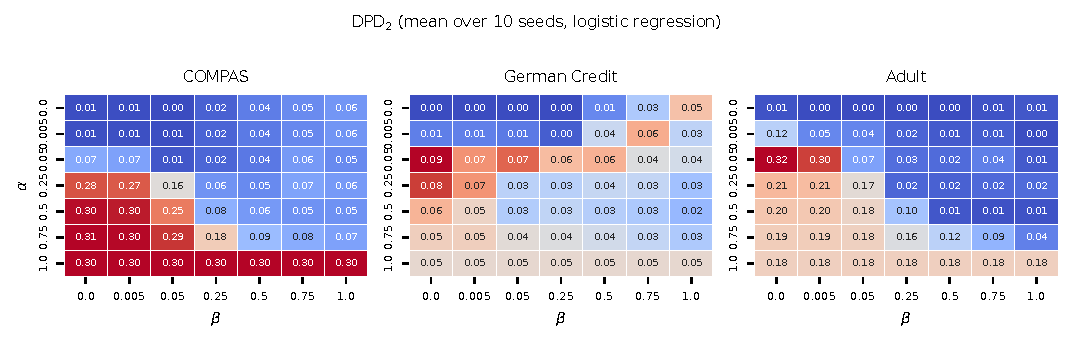
\includegraphics[width=\columnwidth]{heatmap_dpd.pdf}
\caption{\dpdtwo{} over the $\alpha \times \beta$ grid (mean over ten seeds,
logistic regression). Disparity falls as $\beta$ increases, most strongly at
intermediate $\alpha$.}
\label{fig:heatdpd}
\end{figure}

\begin{figure}[t]
\centering
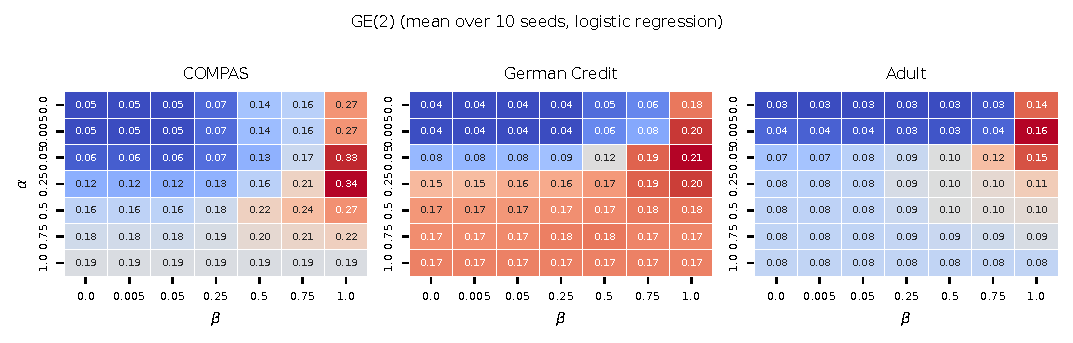
\includegraphics[width=\columnwidth]{heatmap_ge.pdf}
\caption{\getwo{} over the same grid. The gradient runs in the opposite
direction to Fig.~\ref{fig:heatdpd} across $\beta$, which is the double
dissociation viewed as a surface.}
\label{fig:heatge}
\end{figure}

\section{Discussion}
\label{sec:discussion}

\subsection{Why the Two Objectives Are Not Symmetric}

The group term moves its target by roughly $80\%$; the individual term moves
its own by roughly $5\%$. The asymmetry is not a tuning artefact but follows
from what each objective can control.

\softdp{} in \eqref{eq:softdp} is a difference of group means of $p$. A model
can reduce it by shifting the decision surface between groups---an operation
that costs little accuracy because it redistributes predictions rather than
requiring better ones. The quantity is, in effect, freely adjustable.

\softge{} in \eqref{eq:softge} is the inequality of $b_i = 1 + p_i - y_i$.
Benefit equality is attained exactly when $b_i$ is constant, that is when
every individual is predicted equally correctly. Its floor is therefore set by
the irreducible error of the hypothesis class on the data: one cannot equalize
benefit without in fact being more accurate. On COMPAS, where the ceiling is
approximately $0.68$ accuracy, there is little room, and the term accordingly
achieves little. A useful implication is that individual fairness in this
outcome-based sense is not primarily an allocation problem but a
\emph{prediction-quality} problem.

\subsection{$\beta$ as a Policy Parameter, Not a Hyperparameter}

Hyperparameters are tuned: one searches for the value that maximises a
criterion. $\beta$ does not admit that treatment, because the two ends of its
range optimise different criteria and there is no metric that ranks them.
Selecting $\beta$ by validation performance simply encodes whichever fairness
notion the validation metric happens to measure---which is exactly what our
utopia-distance rule does, and why it is scale-sensitive
(Section~\ref{sec:german}).

$\beta$ is better understood as a \emph{policy dial}: it makes explicit a
commitment that is otherwise implicit and undocumented in a deployed system.
Our results give that commitment a price. On Adult, moving from $\beta=0$ to
$\beta=1$ buys a $0.18$ reduction in demographic parity difference at a cost
of $0.22$ in equalized odds difference and $0.015$ in benefit inequality. An
institution that must state which definition it is optimizing can read the
consequences of that choice off the trade-off map rather than discovering them
after deployment.

\subsection{The Uncomfortable Case}

The Adult MLP at $\beta=1$ makes the tension concrete. It achieves
$\dpdtwo = 0.009$: men and women are selected at nearly identical rates, and
by the most widely cited group-fairness definition the model is close to
ideal. The same model has $\mathrm{EOD} = 0.321$, meaning its error rates
differ across sexes by roughly a third---worse than the unconstrained baseline
by a factor of $3.3$. Both statements are true of the same predictor.

There is no analysis internal to the data that resolves this. Whether it is
better to select equally or to err equally is a normative question about what
the decision is for. The value of a trade-off map is not that it answers the
question but that it prevents the answer from being made accidentally, by a
default in a fairness library.

\subsection{Where the Composite Loss Sits Among Existing Methods}

On group-fairness metrics the loss matches rather than beats
Reweighing~\cite{kamiran2012data},
ExponentiatedGradient~\cite{agarwal2018reductions} and
ThresholdOptimizer~\cite{hardt2016equality}
(Table~\ref{tab:master}, Fig.~\ref{fig:pareto}). We regard that as sufficient
for its purpose: an instrument used to measure a trade-off must be credible on
the axis it shares with existing tools, and it is.

Its distinguishing property is the one those methods lack. Each of the
baselines is constructed around a single constraint---demographic parity or
equalized odds---and offers no continuous path to an individual-fairness
objective. The composite loss traverses that path within a fixed architecture,
optimizer and evaluation protocol, so differences along $\beta$ are
attributable to the objective rather than to a change of method. That is what
makes Fig.~\ref{fig:beta} interpretable as a trade-off curve.

\subsection{A Sample-Size Floor for Fairness Model Selection}

The German Credit analysis (Section~\ref{sec:german}) generalizes beyond this
paper. Fairness metrics are differences of \emph{conditional} rates, so their
effective sample size is governed by the smallest group, not by $n$. With
$310$ women in the dataset and roughly $62$ in a validation split, the
standard error of a group selection rate is comparable to the entire disparity
being measured, and validation-based tuning ranks noise
(Table~\ref{tab:selection}).

Practitioners frequently select fairness hyperparameters exactly this way. Our
results suggest that such a procedure should be accompanied by a check---the
validation--test correlation of the fairness metric across configurations is a
cheap one---and that where it fails, a pre-specified configuration is
preferable to a tuned one. The cost of ignoring this is not merely a weaker
result: on German the tuned model reproduced the baseline disparity while a
pre-specified $\beta=1$ reduced it by $48\%$ at no accuracy cost.

\section{Limitations}
\label{sec:limitations}

We state the constraints on these results explicitly, since several bear
directly on how the numbers should be read.

\subsubsection{The individual-fairness notion is outcome-based, not Lipschitz}
We measure individual fairness as inequality of the benefit vector following
Speicher et al.~\cite{speicher2018unified}. This requires no similarity metric,
which is why it is computable here, but it does not establish the
``similar individuals treated similarly'' property of
Dwork et al.~\cite{dwork2012fairness}. Claims in this paper about individual
fairness should be read as claims about the distribution of benefit.

\subsubsection{\getwo{} on hard predictions is a function of the error profile}
With $\hat{y} \in \{0,1\}$ the benefit takes only three values,
$b_i \in \{0,1,2\}$, so \getwo{} is determined by the counts of false
positives and false negatives. It is a legitimate inequality measure of the
error distribution, but it does not distinguish \emph{which} individuals bear
those errors.

\subsubsection{Equalized odds on COMPAS is unreliable}
Unlike \dpdtwo{}, our EOD is computed over all six race groups, two of which
contain $31$ and $11$ individuals in total. The resulting statistic has a
standard deviation of $0.13$--$0.22$ across seeds and no COMPAS EOD comparison
reaches significance. COMPAS EOD values in Tables~\ref{tab:master}
and~\ref{tab:ablation} should be treated as uninformative; a largest-two-groups
EOD would be the appropriate fix and is left to future work.

\subsubsection{German Credit is underpowered}
At $n=1000$ the test split contains $200$ rows and validation-based selection
does not function (Section~\ref{sec:german}). The dataset supports the
pre-specified contrast we report but not tuned model selection.

\subsubsection{Full-batch training}
Because \eqref{eq:softdp} requires every group to be present to form a group
gap, each epoch is one full-batch gradient step, capped at $300$. Mini-batch
behaviour of the composite loss---including whether stochastic group
composition destabilises \softdp{}---is untested and would be required before
applying this at larger scale.

\subsubsection{Fixed threshold}
The differentiable models decide at a fixed $0.5$ threshold, whereas the
ThresholdOptimizer baseline is permitted group-specific thresholds. The
comparison in Table~\ref{tab:master} is therefore not threshold-matched.

\subsubsection{The selection rule embeds a value judgement}
Minimising $\sqrt{(1-\mathrm{acc})^2 + \mathrm{DPD}_2^2}$ treats one point of
accuracy as equal to one point of disparity, and is sensitive to the scale of
each term (Table~\ref{tab:selection}). A different scalarization would select
different models. The ablation results of Section~\ref{sec:rq1}, which fix
$\beta$ rather than selecting it, do not depend on this choice.

\subsubsection{Single, binary sensitive attribute}
Each dataset is analysed with respect to one attribute, and no intersectional
analysis (for example race $\times$ sex on Adult) is performed. Subgroup
fairness is known to behave differently from marginal group
fairness~\cite{kearns2018preventing}.

\subsubsection{Inconsistent positive-class polarity}
The positive class is the adverse outcome on COMPAS and German Credit and the
favourable outcome on Adult. Directions of the fairness metrics are unaffected,
but a statement such as ``group $A$ is selected more often'' has opposite
welfare meanings across datasets.

\subsubsection{Sensitive attribute used as an input}
Retaining the sensitive attribute is deliberate and standard in this setting,
but it is a modelling choice with legal implications in some jurisdictions,
and results may differ where its use is prohibited.

\subsubsection{Adversarial debiasing not evaluated}
All three mitigation families are represented, but a second in-processing
method~\cite{zhang2018mitigating} was not run.

\subsubsection{Scope}
Conclusions are limited to binary classification on tabular data with the
three datasets studied. Benchmark-specific artefacts are
documented~\cite{bao2021its,ding2021retiring,fabris2022algorithmic}, and the
COMPAS leakage correction of Section~\ref{sec:setup} is one such case we
encountered directly.

\section{Conclusion}
\label{sec:conclusion}

We set out to measure, rather than derive, the tension between group and
individual fairness. To do so we built a differentiable composite loss whose
parameter $\beta$ interpolates continuously between a soft demographic-parity
term and a soft generalized-entropy term, and swept it across a $7\times7$
$(\alpha,\beta)$ grid, three datasets, two model families and ten seeds:
$2{,}940$ trained models with paired significance testing throughout.

Three findings stand out. First, the two objectives exhibit a statistically
significant \emph{double dissociation}: the group term reduces demographic
disparity by $78\%$--$89\%$ while significantly worsening benefit inequality,
and the individual term significantly improves benefit inequality while
leaving disparity unchanged or worse. The effects are strongly asymmetric in
magnitude, because equalizing benefit is bounded by the achievable prediction
quality in a way that equalizing selection rates is not. Second, on Adult the
conflict extends within group fairness: driving demographic parity to $0.009$
raises equalized odds by a factor of $3.3$, an empirical instance of a known
impossibility, with the exchange rate quantified. Third, where a baseline
already exhibits little disparity, the intervention has nothing to act on, and
where the dataset is small, validation-based selection cannot reliably find
the configurations that would act---on German Credit the tuned model
reproduced the baseline disparity while a pre-specified configuration reduced
it by $48\%$ at no accuracy cost.

The composite loss reaches group-fairness levels comparable to established
pre-, in- and post-processing methods without surpassing them. That was not
the objective; the objective was a measurement instrument credible on the axis
it shares with existing tools, and one that additionally traverses the axis
they do not.

The practical consequence is that $\beta$ should not be tuned. There is no
metric that ranks its endpoints, because they optimize different and partly
opposed definitions of the same word. It is a policy parameter, and the
contribution of a trade-off map is to attach a measured price to each setting
so that the choice is made deliberately rather than inherited from a library
default.

Future work should extend the map to intersectional subgroups, replace the
all-groups equalized odds statistic with a largest-two-groups variant on
COMPAS, test the composite loss under mini-batch training at larger scale, and
characterise more precisely the sample-size floor below which fairness
model selection ceases to function.


\section*{Reproducibility}
All experiments run on CPU. The complete pipeline---data loading, the
$\alpha\times\beta$ sweep, baselines, significance testing, and every figure
and table in this paper---is reproducible with two commands, and per-seed
result files are written for all $2{,}940$ trained models.

\bibliographystyle{IEEEtran}
\bibliography{refs}

\end{document}
